\chapter{Technical Background}
\label{ch:techbg}
This chapter provides brief explanation on different tools, technologies and drone used for the internship work. The technologies listed in this chapter are used completely or partly in the development and the description for the same is referred from their official documentation and websites.

\section{Robot Operating System}
\label{sec:techbg:ROS}
Robot Operating System\cite{quigley2009ros} or popularly known as ROS, facilitates libraries and development tools to help software engineers to design and develop robot applications. It gives hardware abstraction, low-level device control, device drivers, libraries, visualizers, message-passing etc. ROS is authorized under an open source, BSD licence. ROS is tested extensively on Ubuntu and other Linux distributions. ROS community has developed many extensions for other Linux distributions such as Raspbian, Debian and Jetson platforms. ROS is a distributed framework that enables executable to be individually catered and tailored based on the needs of the developer and the design of the application. ROS also supports docker platform for the ease of virtualization and deliver software in terms of Containers.
\\

A developed software or application can be a node or part of a node which publishes or subscribes to a topic. A channel created between subscriber and publisher is called a topic and messages are exchanged through topics. A “Node” or group of “Nodes” can exist both on remote master PC’s side as well as on the robot’s side. Multiple robots can also use similar way of exchanging data through topics. This type of communication is based on Message Queuing Telemetry Transport (MQTT) which is based on Publisher-Subscriber architecture.For further information about can be found at their wiki page \cite{ROSWiki}.

\section{DJI Matrice 210 RTK v2}
\label{sec:techbg:DJIdrone}
DJI Matrice 210 RTK v2 is the UAV or drone used in our work for the purpose of development and a platform to build applications for the same. DJI Matrice 210 RTK v2 is a drone model is developed and produced by the company DJI. This model comes from their industrial drones series used for various purposes like research, agricultural survey, military, surveillance and monitoring, way-point missions and rescue mission operations. It is one of the most featured drones at the industrial level to count on with rugged aerial platform to oversee tasks and identify threats in the all situations. 

\begin{figure}[h]
    \centering
    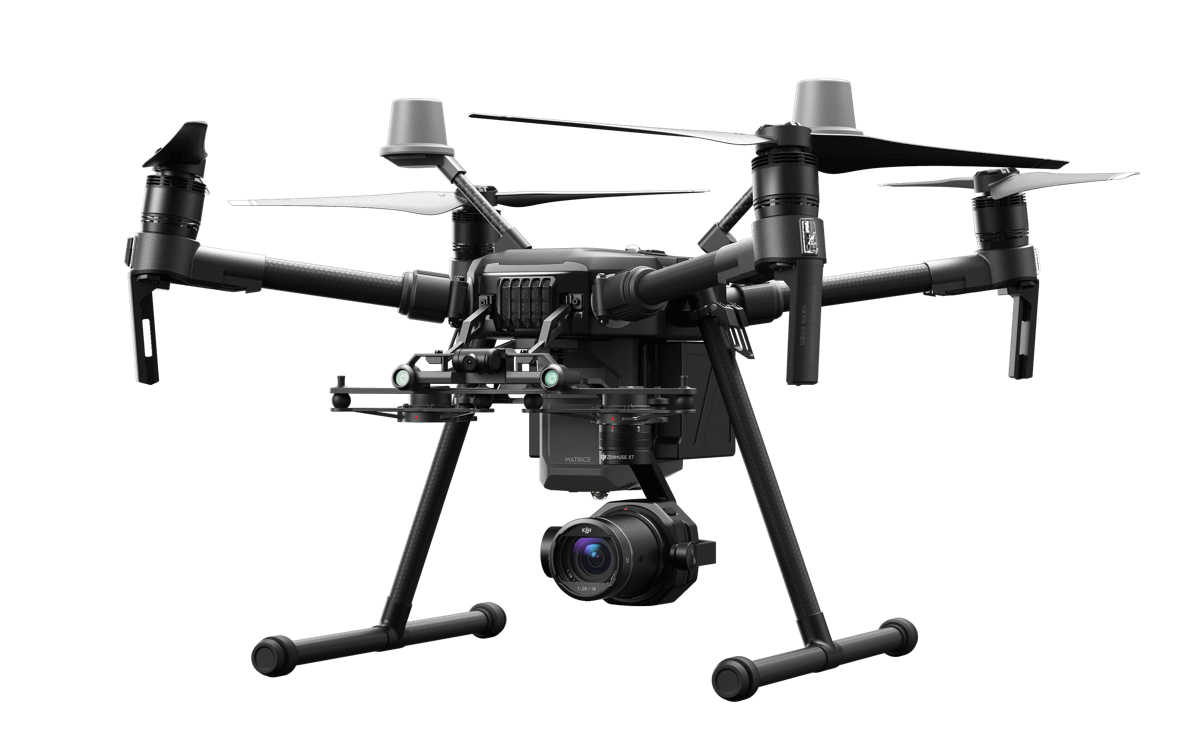
\includegraphics[width=8cm,height=6cm]{Images/drone.png}
    \caption{DJI Matrice 210 RTK v2, Source: DJI website}
    \label{fig:droneimg}
\end{figure}

The main features of the drone are:
\begin{itemize}
    \item Comes installed with Manifold 2, an enterprise version of NVIDIA Jetson TX2 on-board computer which enables the drone to work as autonomous robot with developed software and applications. Manifold 2 runs on Ubuntu 16.04 operating system.
    \item Supports Robot Operating System (ROS) for using drone in the robotic environments.
    \item On-board SDK and ROS On-board-SDK are the open source developer tools offered by DJI. This reduces the burden of creating base packages to communicate with the hardware and adapting the same to ROS environment.
    \item Drone comes with multiple cameras such as front stereo cameras, downward stereo cameras, First Person View (FPV) camera and a high-end payload camera with gimbal. The payload camera is a Zenmuse X5S that comes with a micro 4/3" sensor supporting eight standard M4/3" lenses ranging from 9 mm-45 mm. For our work, the Olympus M.Zuiko 45mm / 1.8 lens was employed. 
    \item Other sensors like IMU sensor, Infrared sensors and Global Navigation Satellite System (GNSS) which supports GPS, GLONASS, BeiDou and Galileo. 
\end{itemize}

\section{ORB-SLAM3}
\label{sec:techbg:orbslam3}
ORB-SLAM is a Simultaneous Localization and Mapping (SLAM) solution for Monocular, Monocular-Inertial, Stereo, and RGB-D cameras. It can compute the camera keyframe trajectory and a sparse 3D reconstruction of the scene in real time in a wide range of scenarios, from small sequence to a vehicle driving around the few city areas. It comes with a robust and automatic initialization from both planar and non-planar scenes. It can close large loops and conduct global re-localization from a wide range of baselines in real time. ORB-SLAM project started off with Monocular Visual SLAM in their first library ORB-SLAM \cite{murAcceptedTRO2015}. They released the next version called ORB-SLAM2 \cite{murORB2} which features Stereo and RGB-D camera based SLAM solution. \\

At present, the ORB-SLAM3 \cite{ORBSLAM3_2020} is the cutting edge release from the same project which features Visual Inertial SLAM i.e Monocular Inertial SLAM solution. ORB-SLAM3 as whole includes all the prior features from ORB-SLAM and ORB-SLAM2. They also claim in their paper \cite{ORBSLAM3_2020} that ORB-SLAM3 is the first system capable of performing visual, visual-inertial and multi-map SLAM with monocular, stereo and RGB-D cameras and supports pin-hole as well as fish-eye models.
This approach is more robust and two to five times accurate than previous approaches. It is also an open-source library, free for all to use for research and development purposes. \\

There are several other Visual SLAM and VI-SLAM libraries as open-source tools such as VINS-Mono \cite{Geneva2020ICRA} and \texttt{open\_vins} \cite{qin2017vins} but for our work we consider ORB-SLAM3 and try to work through it to get the results.

\section{GeographicLib}
\label{sec:techbg:geographiclib}
GeographicLib \cite{GeographicLib} is a simple C++ libray which provides methods for Geodesic conversions, Geoid modeling and gravity and magnetic field calculations. The main highlights of the library is that it supports conversion between Universal Transverse Mercator (UTM), Universal Polar Stereographic (UPS), WGS84 system, Earth Centric Earth Fixed (ECEF) and local coordinate systems like ENU and NED. This library reduces the overhead of developing custom methods to compute the conversion. In this internship, this library is employed in the second latter part of work where we develop a geo-referening node parallel to ORB-SLAM3 custom node. The following methods are used in the development of the node-
\begin{itemize}
    \item WGS84 to ECEF conversion.
    \item WGS84 to ENU conversion.
    \item Creating WGS84 earth model for the reference used in conversions. 
\end{itemize}

\section{Kalibr}
\label{sec:techbg:kalibr}
Kalibr \cite{Kalibr} is a conglomeration of tools for different kinds that help in solving calibration problems. This tool was created by referring to many papers but the main work published is \cite{7487628}. The toolbox offers the following tools-
\begin{itemize}
    \item Multiple camera calibration.
    \item Camera-IMU calibration.
    \item Rolling Shutter Camera calibration.
    \item Other co-supporting tools.
\end{itemize}

In our work, Camera-IMU calibration tool \cite{6696514}\cite{6225005} is used to generate transformation matrix between camera and IMU sensor. 

\vspace{1cm}
Further, we move to new chapter which will explain the initial setup, installation and architecture for the development.   